\section*{Anhang}

\addcontentsline{toc}{section}{Anhang}

\centering

\null\vfill
\begin{figure}
	\centering
	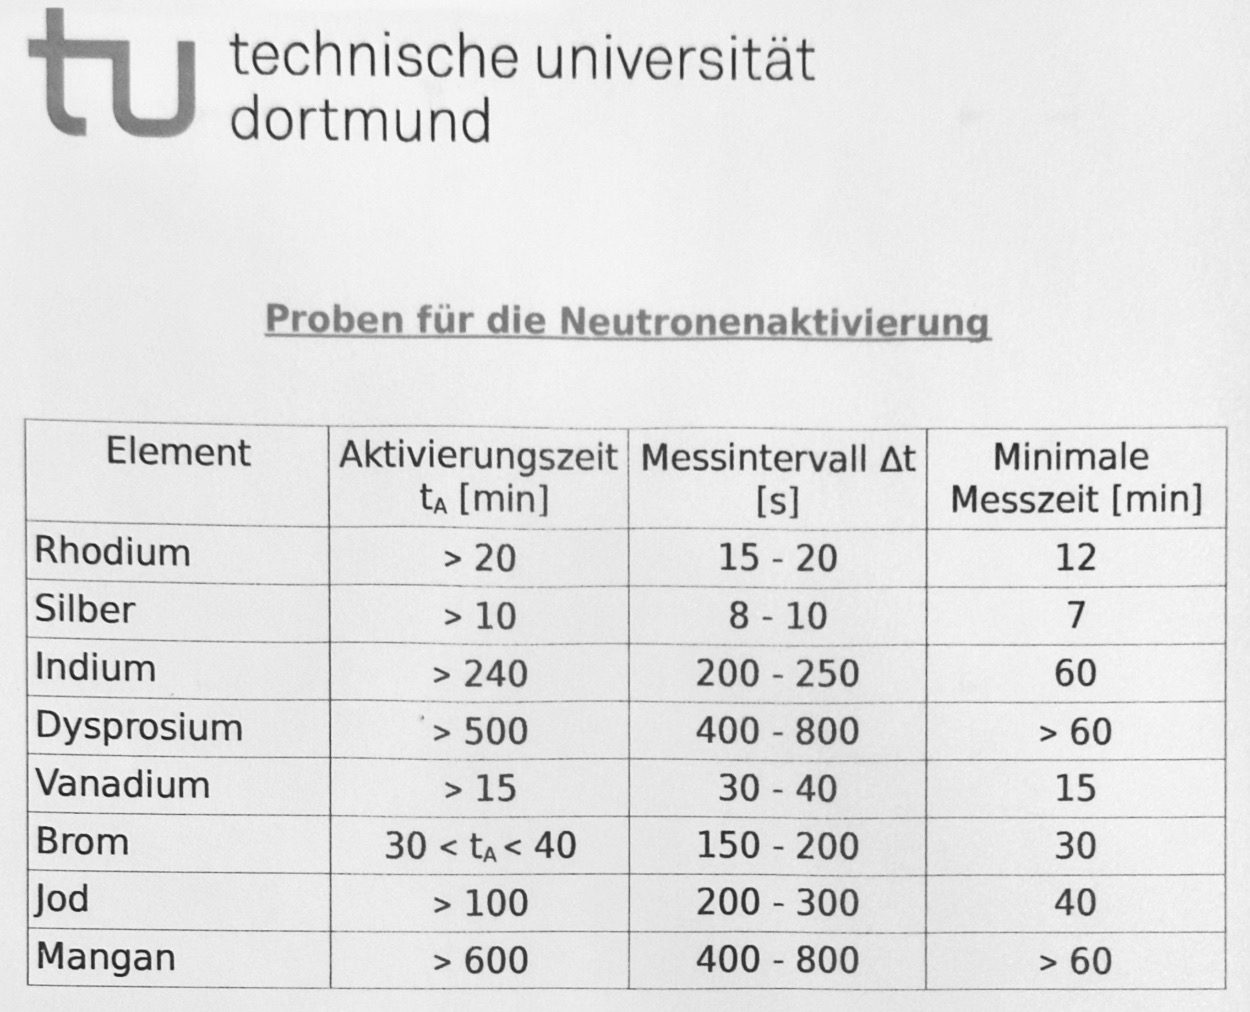
\includegraphics[width=0.5\paperwidth]{content/grafik/liste.jpg}
	\vspace{1ex}
	\caption{Ausgehängte Liste zu Messintervallen und Aktivierungszeiten.}
	\label{fig:liste}
\end{figure}
\vfill\null
\newpage
\null\vfill
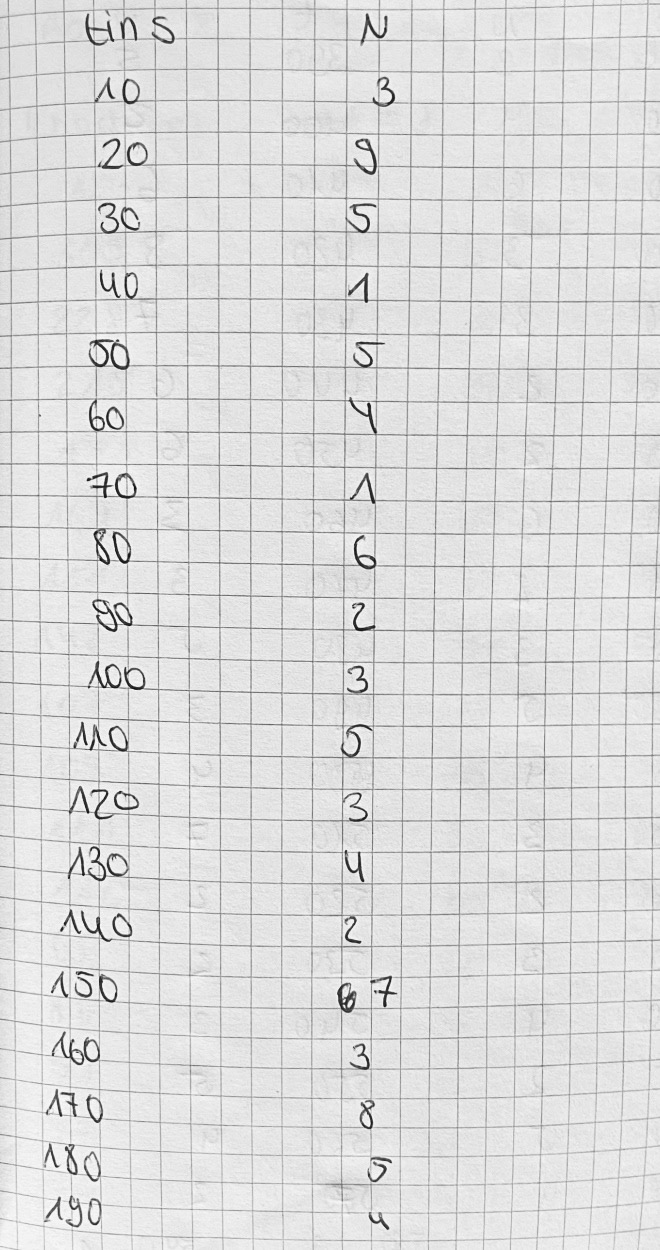
\includegraphics[height=0.5\paperheight]{content/messung/1.jpg}
\vfill\null
\newpage
\null\vfill
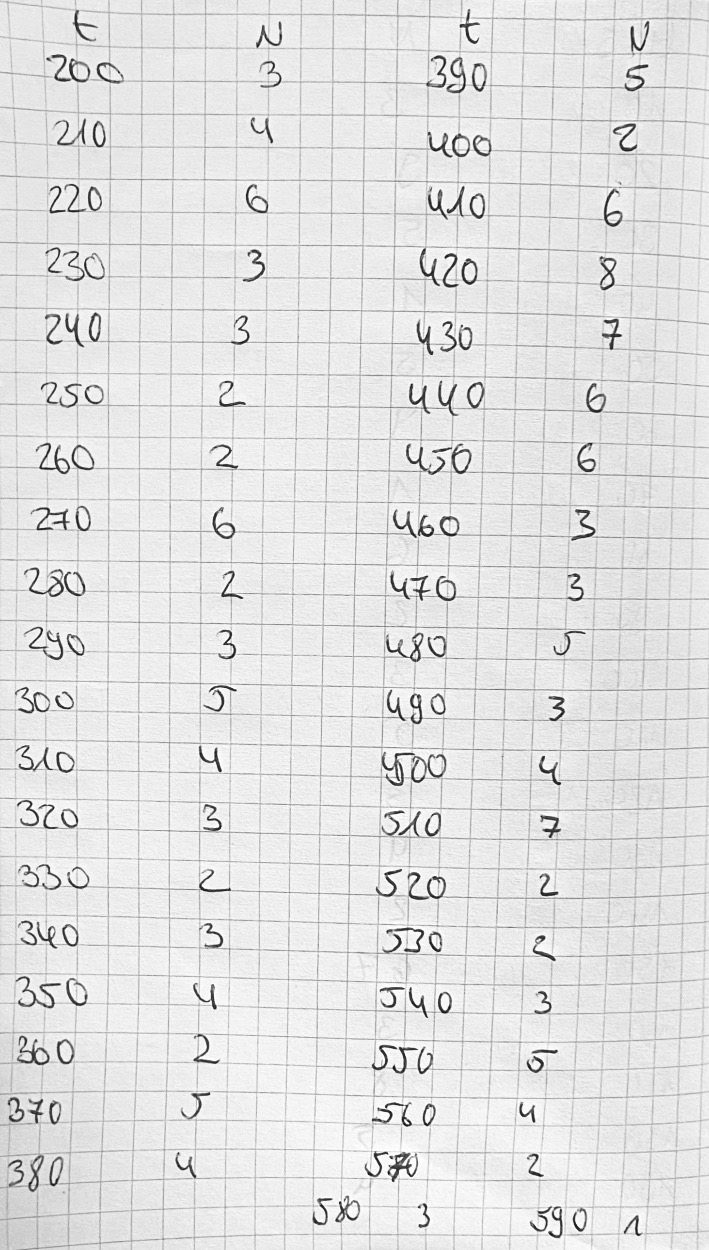
\includegraphics[height=0.5\paperheight]{content/messung/2.jpg}
\vfill\null
\newpage
\null\vfill
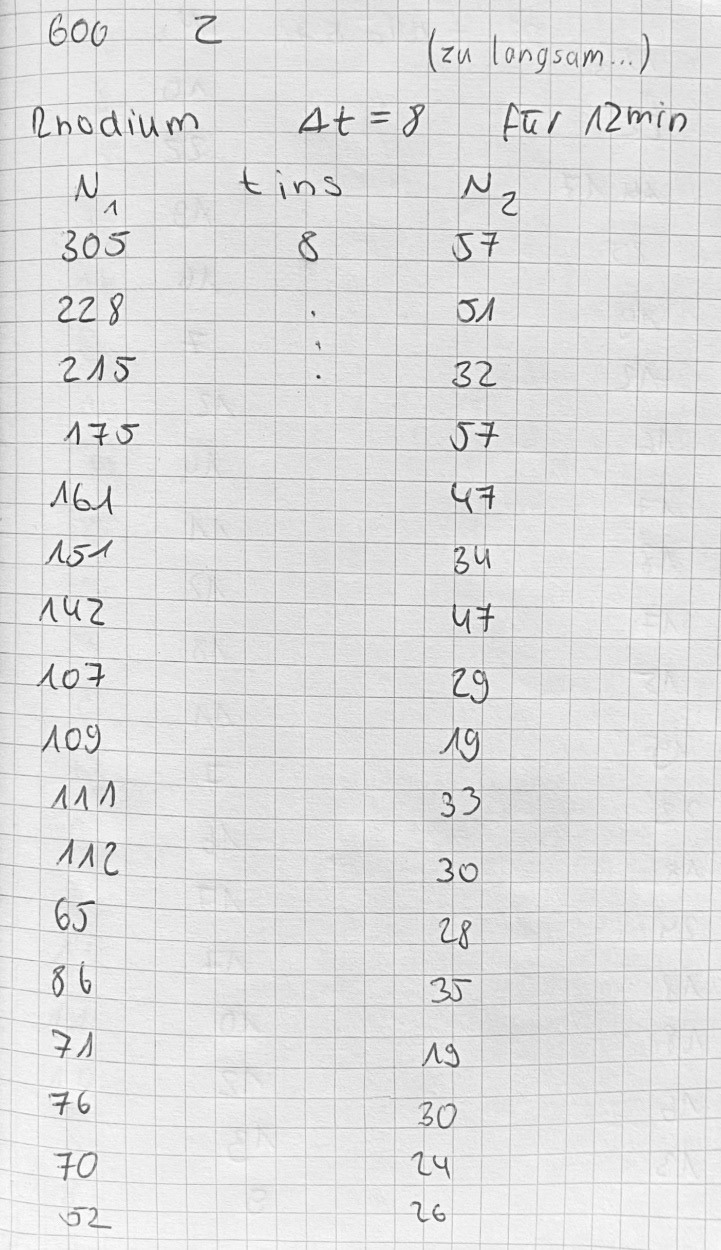
\includegraphics[height=0.5\paperheight]{content/messung/3.jpg}
\vfill\null
\newpage
\null\vfill
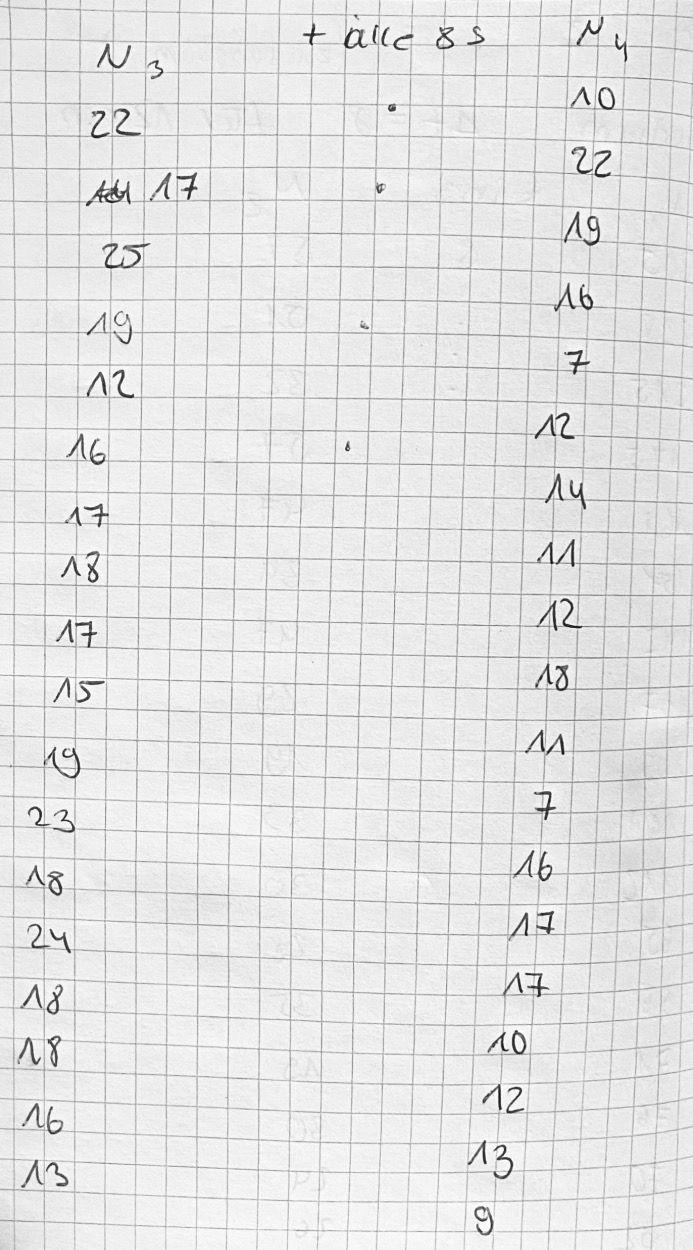
\includegraphics[height=0.5\paperheight]{content/messung/4.jpg}
\vfill\null
\newpage
\null\vfill
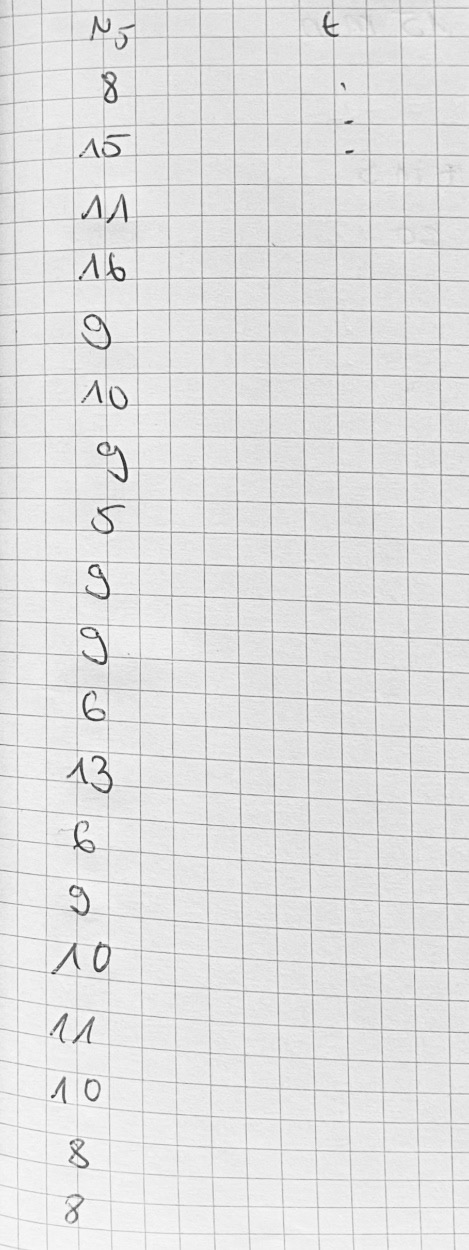
\includegraphics[height=0.5\paperheight]{content/messung/5.jpg}
\vfill\null
\newpage
\null\vfill
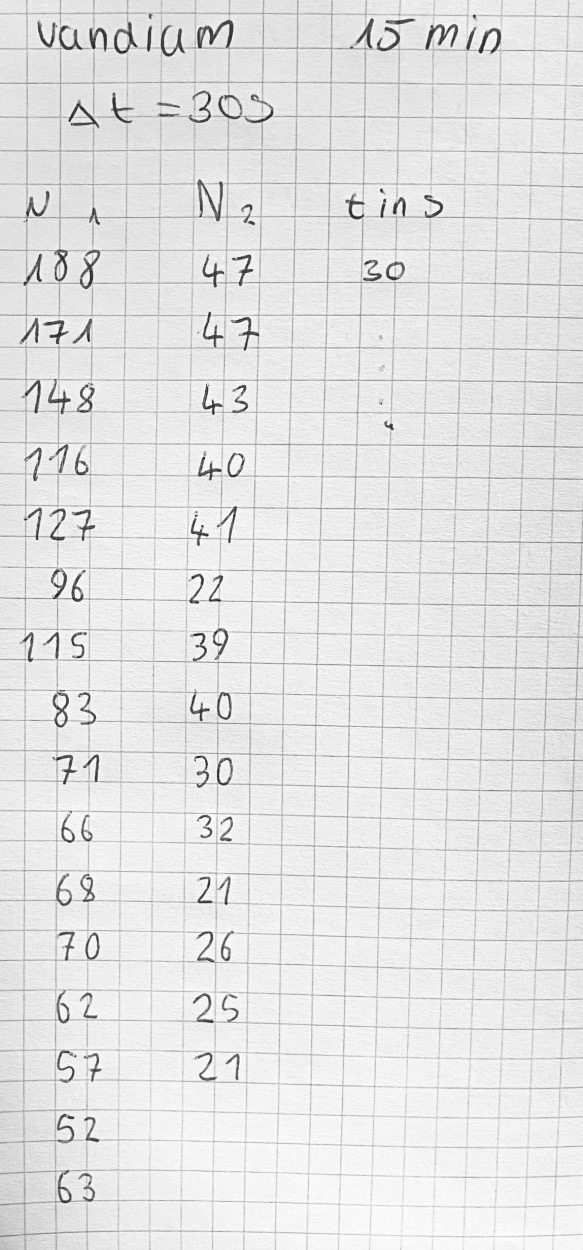
\includegraphics[height=0.5\paperheight]{content/messung/6.jpg}
\vfill\null
\newpage
\null\vfill
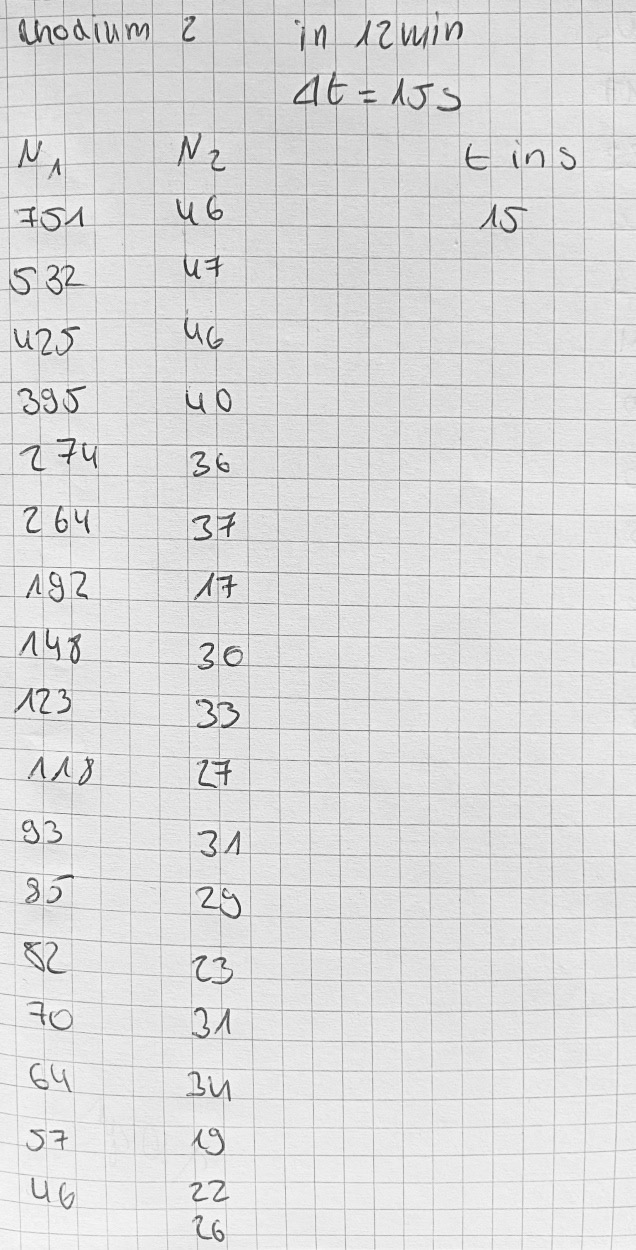
\includegraphics[height=0.5\paperheight]{content/messung/7.jpg}
\vfill\null
\newpage
\null\vfill
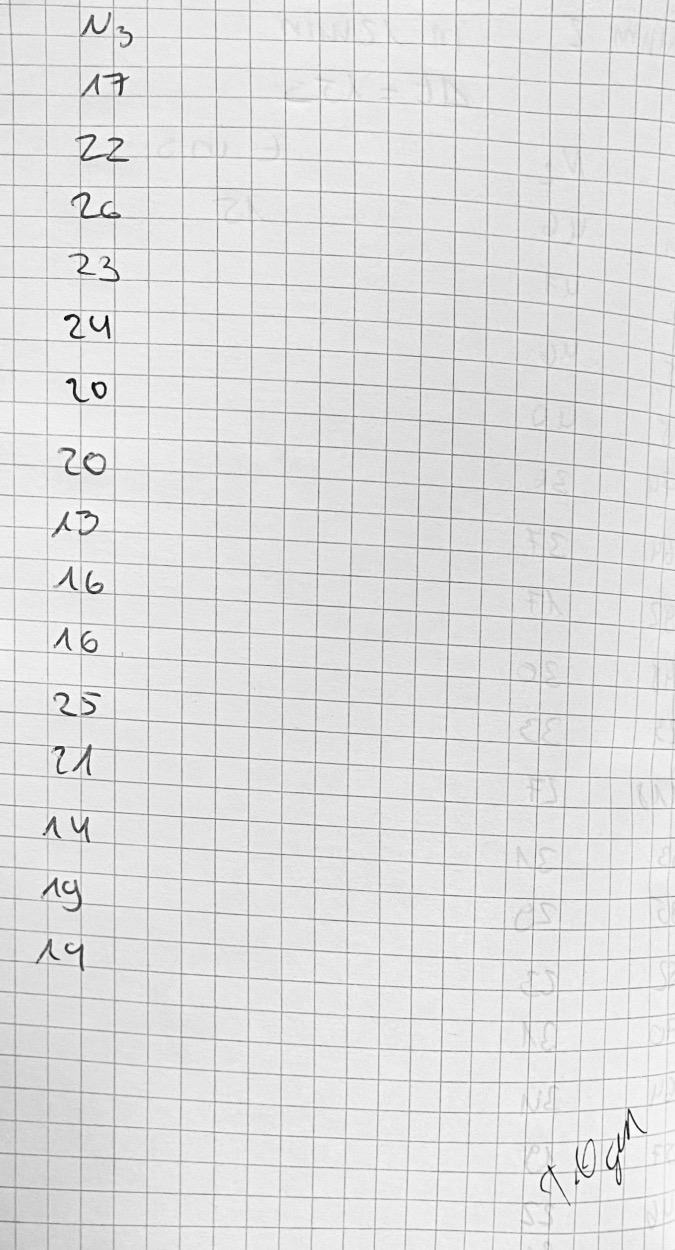
\includegraphics[height=0.5\paperheight]{content/messung/8.jpg}
\vfill\null
